\documentclass{standalone}
\usepackage{tikz}
\usetikzlibrary{bayesnet}

\begin{document}

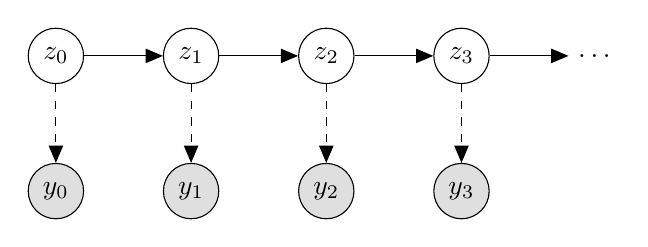
\begin{tikzpicture}
  \node[latent] (z0) {$z_0$};
  \node[latent, right=of z0] (z1) {$z_1$};
  \node[latent, right=of z1] (z2) {$z_2$};
  \node[latent, right=of z2] (z3) {$z_3$};
  \node[right=of z3] (stop) {$\ldots$};

  \edge {z0} {z1};
  \edge {z1} {z2};
  \edge {z2} {z3};
  \edge {z3} {stop};
  
  \node[obs, below=of z0] (y0) {$y_0$};
  \node[obs, below=of z1] (y1) {$y_1$};
  \node[obs, below=of z2] (y2) {$y_2$};
  \node[obs, below=of z3] (y3) {$y_3$};

  \edge[dashed] {z0} {y0};
  \edge[dashed] {z1} {y1};
  \edge[dashed] {z2} {y2};
  \edge[dashed] {z3} {y3};
    
\end{tikzpicture}

\end{document}
